\subsection{Ablation Study}


To evaluate the contribution of individual components within the RiskDreamer framework, we conducted a series of ablation studies. These studies specifically assessed the impact of the entropy and risk-balancing mechanisms, as well as the effect of the online planning horizon on the batch planning process.



\begin{figure*}[!htbp]
    \centering
    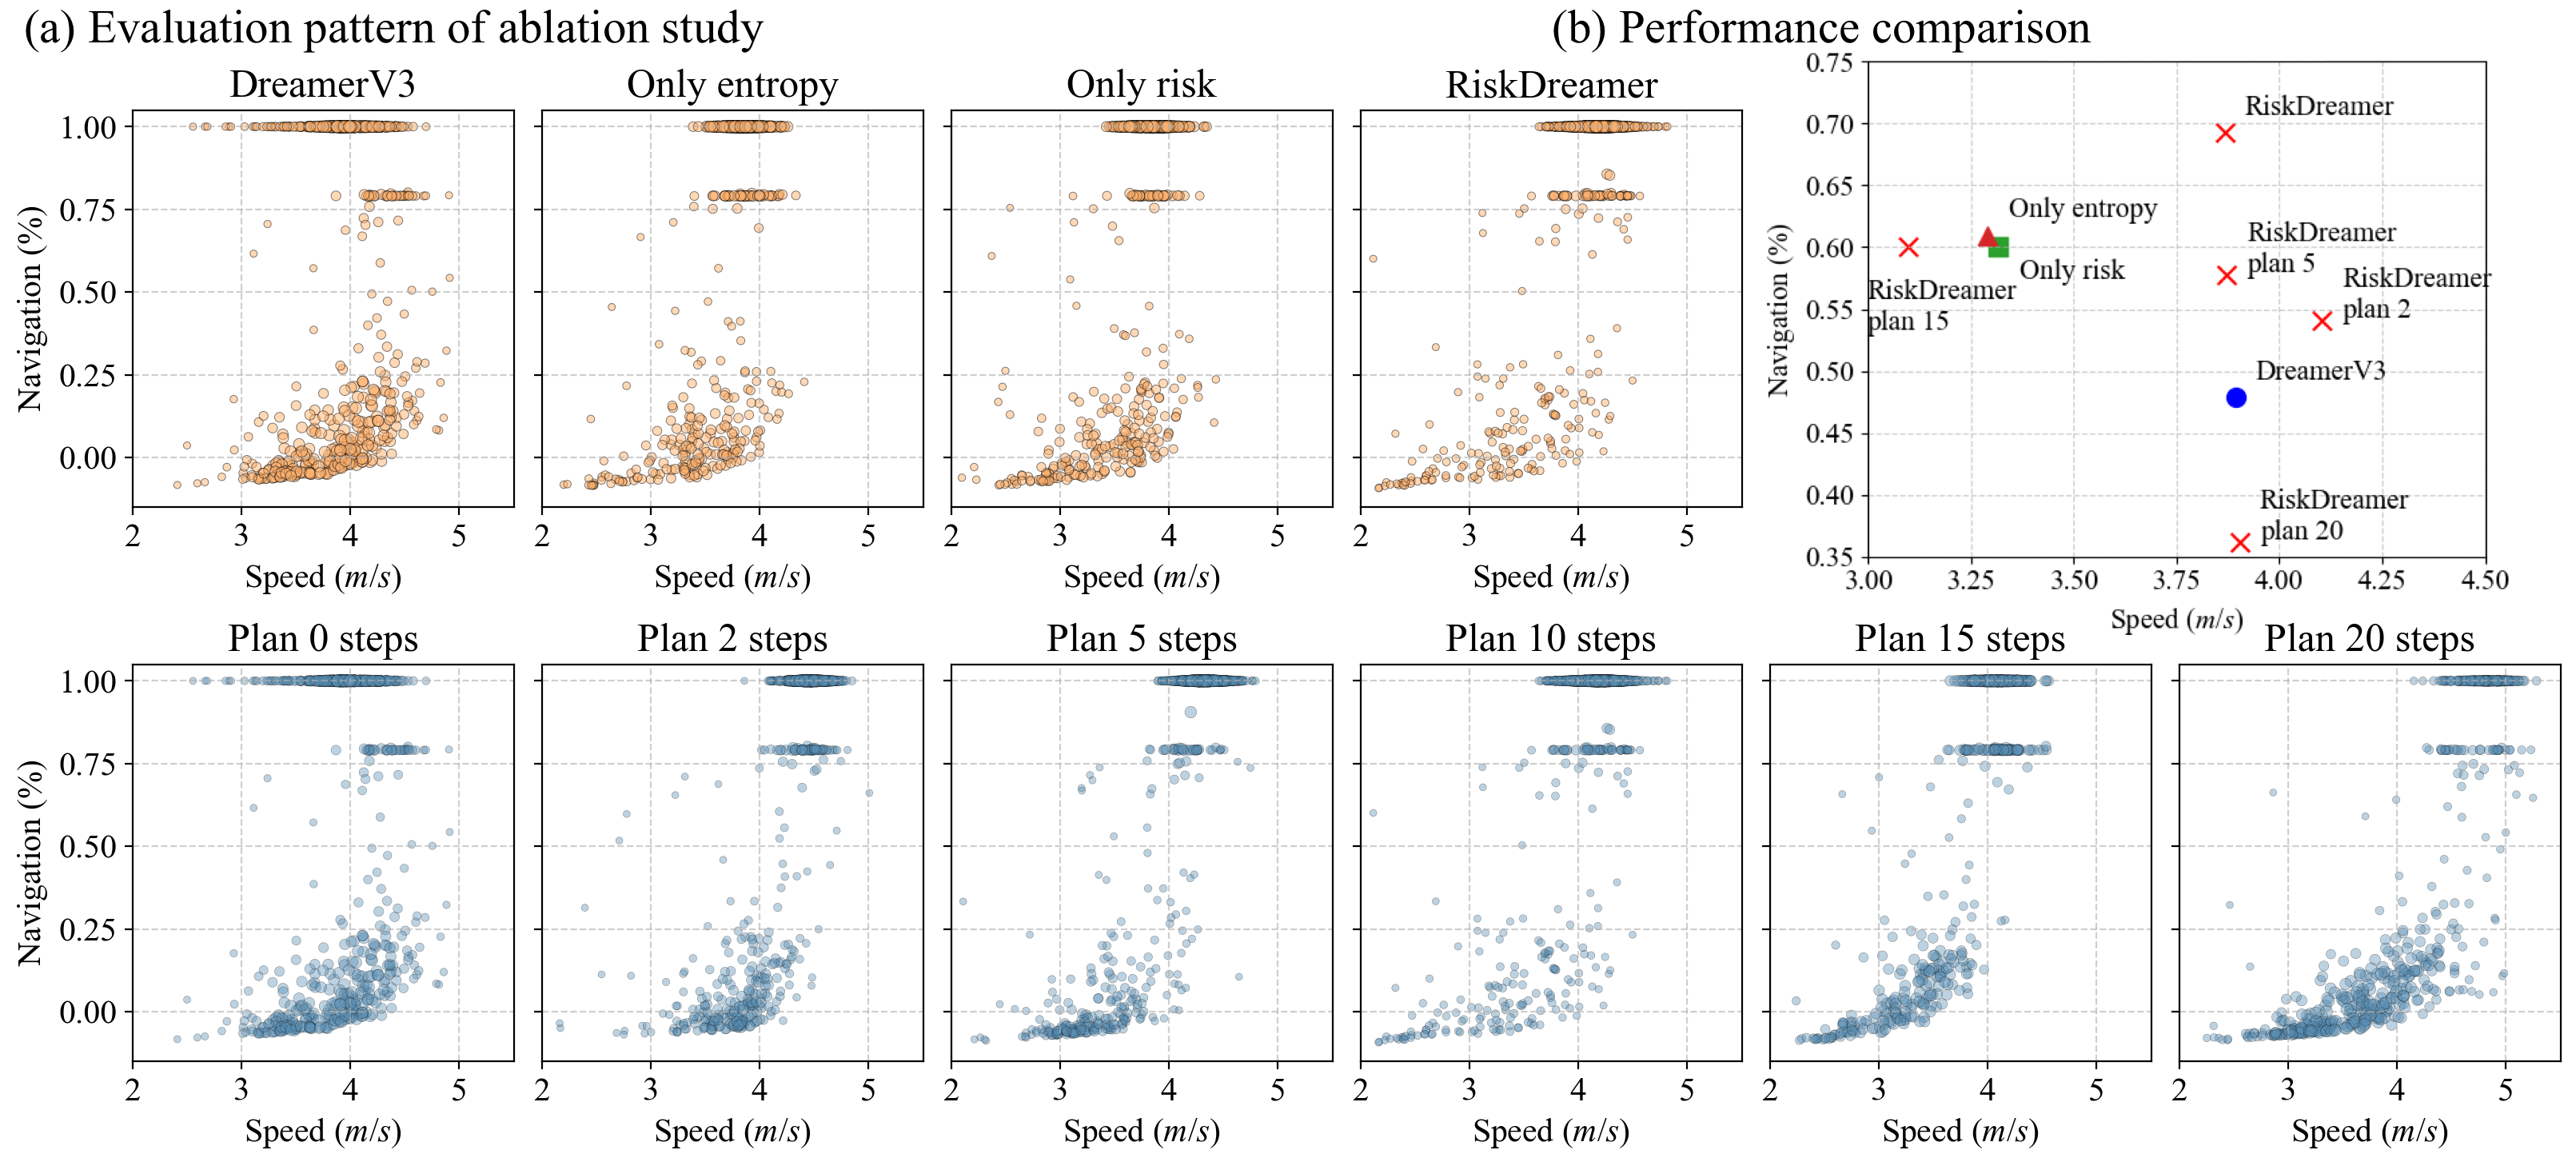
\includegraphics[width=\textwidth]{fig/abafig.png}
    \caption{Results of ablation study (a) Evaluation pattern (b) Performance comparison}
    \label{fig:aba_fig}
\end{figure*}

\begin{table}[!ht]
    \caption{Impact of Entropy and Risk Balancing}
    \label{table:ablation_entropy_risk}
    \centering
    \begin{tabular}{lcccc}
    \toprule
    Algorithm & Speed (Std.) & Navigation (Std.) & Risk (Std.) & Score \\
    \midrule
    \rowcolor{lightgray} RiskDreamer & 3.87 (0.60) & \textbf{0.69} (0.40) & \textbf{0.44} (0.50) & \textbf{0.63} \\
    Only entropy term & 3.29 (0.95) & 0.61 (0.42) & 0.63 (0.48) & 0.55 \\
    Only risk term & 3.32 (0.90) & 0.60 (0.43) & 0.61 (0.49) & 0.54 \\
    DreamerV3 & \textbf{3.89} (0.46) & 0.48 (0.44) & 0.64 (0.48) & 0.48 \\
    \bottomrule
    \end{tabular}
\end{table}



\textbf{Impact of Entropy and Risk Balancing:}
Table \ref{table:ablation_entropy_risk} presents two ablated versions: one using only the entropy balancing term in the action expansion and the other using only the risk balancing term. The full RiskDreamer model achieves the highest overall score (0.63), outperforming both ablated versions and the baseline DreamerV3. RiskDreamer demonstrates superior performance in Navigation (0.69) and Risk (0.44), indicating a more effective balance between task completion and risk mitigation. Although the ablated versions with only entropy or only risk balancing show slightly improved navigation score compared to DreamerV3, they still underperform relative to RiskDreamer and exhibit higher risk values (0.63 and 0.61, respectively). DreamerV3, which does not include explicit entropy or risk balancing, achieves the highest Mean Speed (3.89) but performs poorly in Navigation (0.48) and incurs the highest Risk (0.64), resulting in the lowest overall Score (0.48). Fig. \ref{fig:aba_fig} (a) shows that using only the entropy or risk term reduces the low-speed portion of completed navigation clusters, whereas the full RiskDreamer implementation increases the high-speed portion of these clusters. Fig. \ref{fig:aba_fig} (b) illustrates that both single-term versions produce comparable outcomes by decreasing speed while improving navigation success.

\begin{table}[!ht]
    \caption{Impact of the Number of Planning Branches}
    \label{table:ablation_plan_len}
    \centering
    \begin{tabular}{lcccc}
    \toprule
    Horizon ($H$) & Speed (Std.) & Navigation (Std.) & Risk (Std.) & Score \\
    \midrule
    \rowcolor{lightgray} \textbf{$H$ = 10 (Chosen)} & 3.87 (0.60) & \textbf{0.69} (0.40) & \textbf{0.44} (0.50) & \textbf{0.63} \\
    $H$ = 5 & 3.87 (0.59) & 0.58 (0.44) & 0.54 (0.50) & 0.55 \\
    $H$ = 15 & 3.10 (1.15) & 0.60 (0.41) & 0.75 (0.43) & 0.54 \\
    $H$ = 2 & \textbf{4.10} (0.50) & 0.54 (0.44) & 0.60 (0.49) & 0.53 \\
    $H$ = 0 & 3.89 (0.46) & 0.48 (0.44) & 0.64 (0.48) & 0.48 \\
    $H$ = 20 & 3.90 (0.87) & 0.36 (0.40) & 0.80 (0.40) & 0.40 \\
    \bottomrule
    \end{tabular}
\end{table}

\textbf{Influence of Planning horizon length:}
We further investigated the impact of the length of planning horizons employed in our batch planning approach. Table \ref{table:ablation_plan_len} shows RiskDreamer's performance under different planning horizon lengths, ranging from 0 (equivalent to DreamerV3's single-step action selection) to 20. The results indicate that the length of planning horizon significantly affects performance. RiskDreamer with a planning length of 10, our chosen configuration, achieved the best overall Score (0.63), Navigation (0.69), and Risk (0.44). Reducing the planning length to 5 still maintains a competitive Mean Speed (3.87) but leads to a noticeable decrease in Navigation (0.58) and an increase in Risk (0.54), resulting in a lower Score (0.55). Conversely, increasing the planning length beyond 10, such as to 15 and 20, results in degradation of all metrics except for Mean Speed in the case of plan = 20. Specifically, with planning lengths of 15 and 20, we observe a significant increase in Risk (0.75 and 0.80 respectively) and a substantial drop in Navigation (0.60 and 0.36 respectively), leading to lower Scores (0.54 and 0.40). Interestingly, while a very short planning length of 2 leads to the highest Mean Speed (4.10), it also results in compromised Navigation (0.54) and Risk (0.60), and a lower Score (0.53) compared to plan = 10. The case with plan length 0, which is equivalent to acting without planning (similar to DreamerV3), yields the lowest Score (0.48). As shown in Fig. \ref{fig:aba_fig} (a) Evaluation pattern, even plan 2 steps can reduce linear clustering in the low-speed region, with bottom collision clustering being an exception. Furthermore, except for step 15, the model's performance speed tends to increase as steps increase. Fig. \ref{fig:aba_fig} (b) Performance comparison shows increased navigation for all except plan 20.


